\documentclass[tikz,border=10pt]{standalone}
% Regenerate the web asset from this directory with:
%   pdflatex -interaction=nonstopmode -halt-on-error lid_driven_cavity.tex
%   inkscape --pdf-poppler --export-text-to-path \
%     --export-filename=lid_driven_cavity.svg lid_driven_cavity.pdf
\usepackage{amsmath}
\usetikzlibrary{arrows.meta,calc}

\definecolor{domainfill}{HTML}{EDF5FA}
\definecolor{wallcolor}{HTML}{34495E}
\definecolor{lidcolor}{HTML}{C4473A}
\definecolor{textcolor}{HTML}{253746}

\begin{document}
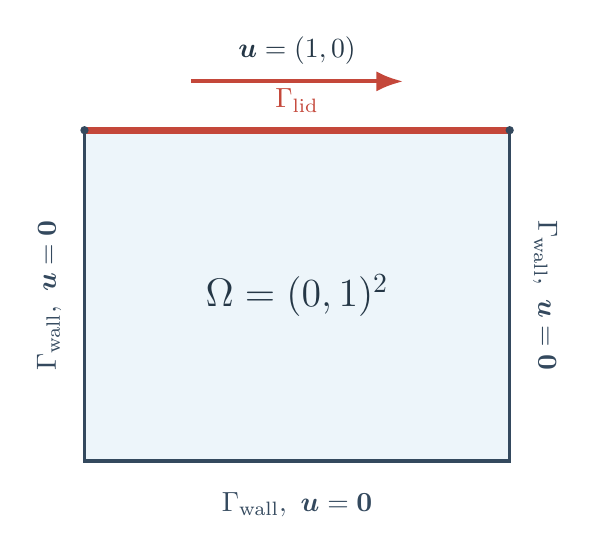
\begin{tikzpicture}[
  >=Latex,
  every node/.style={font=\sffamily, text=textcolor},
  wall/.style={draw=wallcolor, line width=1.2pt},
  lid/.style={draw=lidcolor, line width=2.4pt}
]
  \coordinate (SW) at (0,0);
  \coordinate (SE) at (5.4,0);
  \coordinate (NE) at (5.4,4.2);
  \coordinate (NW) at (0,4.2);

  \fill[domainfill] (SW) rectangle (NE);
  \draw[wall] (NW)--(SW)--(SE)--(NE);
  \draw[lid] (NW)--(NE);

  \draw[lidcolor, line width=1.5pt, ->]
    ($(NW)+(1.35,0.62)$)--($(NE)+(-1.35,0.62)$)
    node[midway, above=2pt] {$\boldsymbol u=(1,0)$};

  \node[lidcolor, above=3pt] at ($(NW)!0.5!(NE)$)
    {$\Gamma_{\mathrm{lid}}$};
  \node[rotate=90, wallcolor] at ($(NW)!0.5!(SW)+(-0.45,0)$)
    {$\Gamma_{\mathrm{wall}},\ \boldsymbol u=\boldsymbol 0$};
  \node[rotate=-90, wallcolor] at ($(NE)!0.5!(SE)+(0.45,0)$)
    {$\Gamma_{\mathrm{wall}},\ \boldsymbol u=\boldsymbol 0$};
  \node[wallcolor, below=8pt] at ($(SW)!0.5!(SE)$)
    {$\Gamma_{\mathrm{wall}},\ \boldsymbol u=\boldsymbol 0$};

  \node[font=\Large\sffamily] at ($(SW)!0.5!(NE)$)
    {$\Omega=(0,1)^2$};

  \fill[wallcolor] (NW) circle (1.5pt);
  \fill[wallcolor] (NE) circle (1.5pt);
\end{tikzpicture}
\end{document}
